\begin{center}
        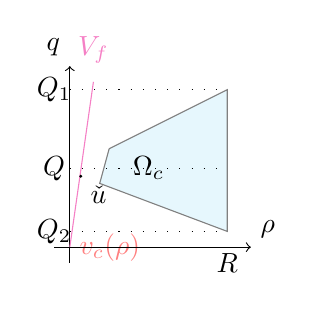
\begin{tikzpicture}
        % coordinates
        \draw[->] (0,-0.2) -- (0,2.3) node[anchor=south east] {$q$};
        \draw[red!50, domain=0:0.7]  plot[id=x] function{x*(3*x+1)}  node[right] {$v_c(\rho)$};
        \draw[magenta!50] (0,0) -- (0.3,2.1);
        \node[magenta!50] at (0.3,2.5) {$V_f$};
        \filldraw[black] (0.14,0.9) circle (0.3pt) node[anchor = north west]{$\check u$} ;
         \filldraw[fill=cyan!10!white, draw=black!50] plot [tension = 1] coordinates { (0.5,1.25) (2,2) (2,0.2) (0.38, 0.81) (0.5,1.25)};
         \node at (1,1) {$\Omega_c$};
         \draw[->] (-0.2,0) -- (2.3,0) node[anchor=south west] {$\rho$};
        \node at (2,-0.2) {$R$};
         \node at (-0.2,2) {$Q_1$};
         \node at (-0.2,0.2) {$Q_2$};
         \node at (-0.2,1) {$Q$};
         \draw[loosely dotted] (0,1) -- (2,1);
         \draw[loosely dotted] (0,2) -- (2,2);
         \draw[loosely dotted] (0,0.2) -- (2,0.2);
       \end{tikzpicture}
    \caption{Domain  $\Omega_c$}
    \label{fig:ConservationLaws/I}
    \end{center}